% **************************** Define Graphics Path **************************
\graphicspath{{Chapter2/Figs/}}

\chapter{Estado del arte}
En este capítulo se presentan los resultados de la investigación del estado del arte. La sección 2.1 está dedicada a introducir conceptos previos que son claves para entender el trabajo. La sección 2.2 estudia las diferentes aplicaciones que se le puede dar a las redes definidas por software, haciendo hincapié en la implementación de redes privadas virtuales. Por último, la sección 2.3 hace un estudio de las diferentes herramientas que se pueden utilizar para virtualizar SDN, y en particular, la arquitectura RAUFlow.

\section{Conceptos previos}
A continuación se explican algunos conceptos que son fundamentales, ya que son sobre los que se basa el proyecto RRAP \cite{proyecto-rrap} y este trabajo. Además, se hace un resumen de los aspectos técnicos de la arquitectura RAUFlow/RAUSwitch.

\subsection{Software Defined Networking}
Las Redes Definidas por Software (o Software Defined Networking en inglés) es una arquitectura de red que propone la separación del plano de control del plano de datos.

Introduce una entidad llamada controlador que centraliza toda la inteligencia de la red. 

\begin{figure}[h] 
	\centering    
	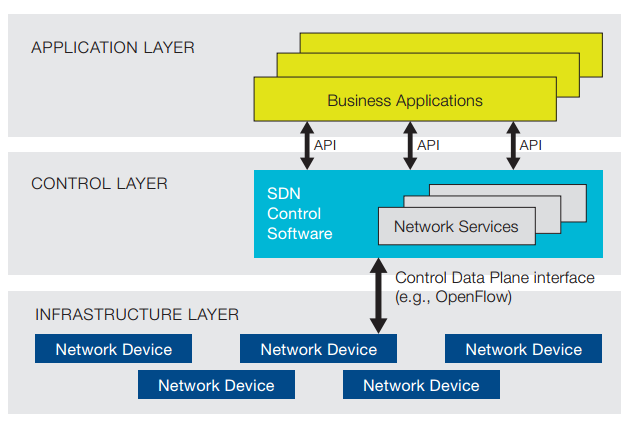
\includegraphics[width=10cm]{arquitectura_sdn}
	\caption{Capas de la arquitectura de SDN. Imagen extraída de \cite{proyecto-rrap}}
	\label{fig:arquitectura_sdn}
\end{figure}

SDNRG
ONF




%https://www.necam.com/docs/?id=2709888a-ecfd-4157-8849-1d18144a6dda

%http://www.iaria.org/conferences2014/filesICNS14/InfoSys%202014%20Control%20Plane%20Scalability%20in%20SDN-%20%20v1.2.pdf

%http://arxiv.org/pdf/1408.6760.pdf

%Ventaja encontrada: puede reducir el procesamiento que se debe hacer en los dispositivos, y eso reduce costos operacionales y aumenta el rendimiento de la red.
%%OPEN promises to reduce the Total Cost of Ownership of  various network  infrastructures  in  part  by  simplifying  the  datapath  switches;  it  provides  greater  control  to  the  operator  to customize and optimize their networks for the features they need and the services they provide; and finally it allows innovation to take place at a much faster rate, by  helping the network evolve  more rapidly in software (implemented outside-the-box), with possibly greater diversity of solutions generated by a larger pool of developers.
%%In today’s packet switched networks, a router is  both  the  control  element  which  makes  control  decisions  on  traffic routing,  as  well  as  the  forwarding element  responsible  for forwarding packets,  and  both  these  functionalities  are tightly linked (Fig.  1a). Housing  control and data functions in the same box necessarily complicates the equipment, which aside from making routing decisions and switching packets, also needs to have all the intelligence necessary for  aggregating  and  disseminating  routing  information, using fully  distributed  routing protocols like OSPF or IS-IS. Furthermore, in IP/MPLS networks, another layer of complexity is added with the need for distributed signaling and label  distribution mechanisms like  RSVP-TE and LDP. Within  a  domain,  an  IP/MPLS  network  may additionally support a host of other protocols such as iBGP, RIP, LMP, SNMP and MP-BGP together  with  many  more protocols for multicast and IPv6. All of these features contribute to control plane load, increased fragility and increased cost (FUENTE: el parrafo anterior y este son del ultimo paper de las vpns sobre SDN)

\subsection{OpenFlow}
Aspectos generales
%http://article.sciencepublishinggroup.com/pdf/10.11648.j.ajsea.20140306.12.pdf

%http://www.spirent.com/~/media/White%20Papers/Broadband/PAB/OpenFlow_Performance_Testing_WhitePaper.pdf

\subsection{Open vSwitch}
%http://openvswitch.org/pipermail/discuss/2012-February/006447.html

%http://openvswitch.org/support/dist-docs/ovs-vswitchd.8.txt

%http://benpfaff.org/papers/ovs.pdf

%http://networkheresy.com/2014/11/13/accelerating-open-vswitch-to-ludicrous-speed/

%http://bluesy.wang/notes/2014/09/14/flow-caching-for-high-entropy-packet-fields/

%http://yuba.stanford.edu/~nickm/papers/flow-caching.pdf

%http://wangcong.org/2012/10/20/an-overview-of-openvswitch-implementation/

%https://www.google.com/url?sa=t&rct=j&q=&esrc=s&source=web&cd=1&ved=0ahUKEwixpuyBieLLAhUCdR4KHVV7CKgQFggfMAA&url=https%3A%2F%2Fnsrc.org%2Fworkshops%2F2014%2Fnznog-sdn%2Fraw-attachment%2Fwiki%2FAgenda%2FOpenVSwitch.pdf&usg=AFQjCNFg9VULvEmHMXQAsuTOE6XLH6WbzQ&bvm=bv.117868183,d.dmo&cad=rja

%http://openvswitch.org/slides/OpenStack-131107.pdf

%http://openvswitch.org/slides/openvswitch.en-2.pdf

%https://www.google.com/url?sa=t&rct=j&q=&esrc=s&source=web&cd=3&ved=0ahUKEwjP95D9ieLLAhVIpB4KHUKeCzYQFggoMAI&url=http%3A%2F%2Fopenvswitch.org%2Fsupport%2Fovscon2014%2F17%2F1530-ovsconf2014_chadnorgan.pptx&usg=AFQjCNEmnrXDB0psj5oXvoAzVYr8F5sLtQ&cad=rja

%https://www.google.com/url?sa=t&rct=j&q=&esrc=s&source=web&cd=1&cad=rja&uact=8&ved=0ahUKEwjZvdvaiuLLAhWF1h4KHfYrCKoQFggiMAA&url=http%3A%2F%2Fopenvswitch.org%2Fsupport%2Fovscon2014%2F18%2F1600-ovs_perf.pptx&usg=AFQjCNGGTT0rHmENeZ2ZcoRfWNFJ__hBLw

\subsection{Multiprotocol Label Switching (MPLS)}
Conceptos básicos

\subsection{Red Privada Virtual (VPN)}
Conceptos básicos

\subsection{RAUFlow/RAUSwitch}

\section{Aplicaciones de SDN}
El paradigma SDN, por definición, está basado en el software. Esto implica que el rango de aplicaciones o modos de uso que se le puede dar al paradigma es enorme. En esta sección se estudiarán algunas aplicaciones existentes sobre SDN, haciendo foco en la implementación de redes privadas virtuales, debido a que es el servicio que provee RAUFlow.
\subsection{Implementación de VPNs}
El desarrollo de redes privadas virtuales (VPN) es un tema de investigación relativamente común en SDN, ya que es un servicio de gran demanda en el mundo actual. A continuación se estudiarán algunas implementaciones existentes de VPN sobre SDN. \\ \\
\textbf{Proyecto CoCo} \\
CoCo \cite{coco-paper} es un proyecto que estudia el desarrollo de un servicio de VPN multipunto enfocado hacia investigadores, para permitirles intercambiar información de modo confiable y seguro. Uno de sus principales enfoques es la facilidad de uso, lo cual es una ventaja frente a las implementaciones tradicionales (no SDN) de este servicio. Sólo requiere que el administrador haga una configuración inicial de la red, y luego los usuarios finales pueden crear, modificar y  eliminar VPNs a demanda mediante un portal web. \\ \\
\begin{figure}[t]
	\caption{Arquitectura de CoCo. Imagen extraída de \cite{coco-paper}}
	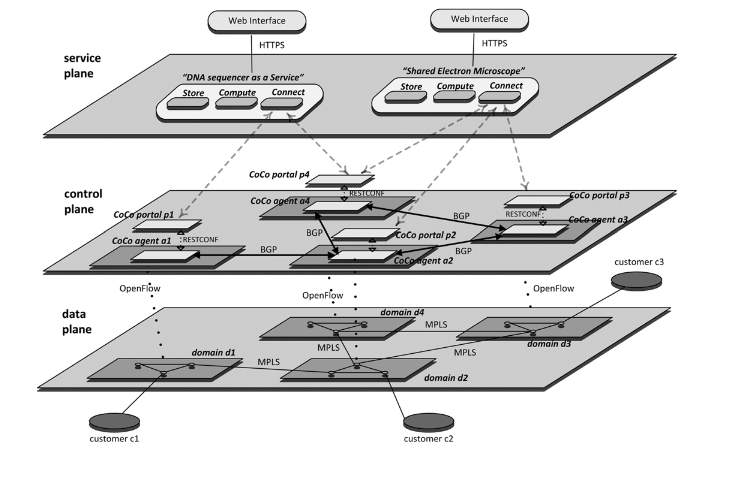
\includegraphics[scale=0.65]{coco_imagen}
	\centering
	\label{fig:coco_imagen}
\end{figure}
La arquitectura de CoCo, que se ilustra en la figura \ref{fig:coco_imagen}, está diseñada para aplicarse a muchos dominios. Cada dominio es una red OpenFlow administrada por un controlador OpenDaylight, llamado agente CoCo. Este último tiene dos grandes tareas. La primera es controlar los switches OpenFlow de su dominio, haciendo descubrimiento de la topología y configurando las reglas de reenvío de los switches. La segunda tarea es en el plano de control de la arquitectura, y consiste en utilizar el protocolo BGP para intercambiar información de accesibilidad con otros agentes CoCo (por ende, otros dominios). \\ \\
Como ya se mencionó, la red de cada dominio está compuesta por switches OpenFlow. Éstos últimos pueden ser internos o de borde, también llamados Provider Edge (o PE). Los de borde son los que se conectan con otros dominios o con las redes cliente (Customer Edge). Las reglas de reenvío están basadas en MPLS, y se utilizan dos niveles de etiquetas. La etiqueta exterior sirve para identificar al switch PE al cual se debe enviar un paquete. La etiqueta interior identifica a la VPN a la cual pertenece el paquete. Esto quiere decir que el tráfico que se recibe por la red CE es etiquetado apropiadamente por el switch PE que recibe dicho tráfico. Cuando el tráfico sale de la red interna hacia la red CE, el switch PE se encarga de remover las etiquetas MPLS del tráfico saliente. \\ \\
\textbf{OpenFlow para mejorar la escalabilidad de un servicio IP-VPN} \\
En \cite{ip-vpn-bgp-sdn} se estudia el problema de la escalabilidad al proveer un servicio de IP-VPN, y propone una solución basada en SDN y OpenFlow. Si un proveedor de servicios de telecomunicaciones ofrece un servicio de IP-VPN, es posible que lo haga utilizando el protocolo BGP. Dicho protocolo se utiliza para intercambiar la información de ruteo correspondiente a cada red cliente conectada al servicio. En un esquema no SDN, el procesamiento del plano de control (en este caso BGP) queda a cargo de los routers de la red. Esto presenta un posible problema de escalabilidad. Cuando se agregan nuevos clientes a la VPN, la nueva información de ruteo debe ser propagada. Los recursos de CPU y memoria de los routers serán consumidos de acuerdo a lo que exijan los nuevos clientes. Por lo tanto, es necesario confirmar que hay margen en la capacidad de los dispositivos antes de aceptar nuevos clientes. \\ \\
La solución que se propone para atacar este problema es utilizar OpenFlow. Se despliega un controlador OpenFlow que además ejecuta múltiples demonios BGP, uno por cada cliente. Los demonios BGP se encargan del intercambio de información de ruteo con los routers de las redes cliente. Un cliente puede tener múltiples redes conectadas a la VPN. Cuando el controlador recibe información de ruteo correspondiente a una determinada red, el demonio BGP encargado de ese cliente notifica a las demás redes del mismo cliente. Además, la misma información de ruteo recibida es procesada para generar las reglas de forwarding (entradas de flujos en los switches OpenFlow) que aseguren la conectividad. Dado que distintos clientes pueden compartir direcciones IP, es necesario que la red OpenFlow pueda distinguir de algún modo a qué cliente pertenece el tráfico. Esto lo logra asignando etiquetas de VLAN a los paquetes cuando entran a la red, que identifican a cada cliente. En el trabajo se menciona, como objetivo futuro, utilizar MPLS en lugar de etiquetas de VLAN. \\ \\
Con la utilización de OpenFlow se resuelve en gran medida el problema de la escalabilidad, ya que se saca el procesamiento del protocolo BGP de los routers y se concentra todo en el controlador. Si bien agregar nuevos clientes a la VPN aumentará la carga de procesamiento y memoria, el controlador puede manejarlo más fácilmente que los dispositivos de red, que tienen recursos mucho más limitados. \\ \\
\textbf{SDxVPN} \\
SDxVPN \cite{sdxvpn} es una propuesta de implementación de VPNs de capa 2 y 3, basadas en MPLS y OpenFlow. Intenta atacar tres problemáticas comunes que experimentan los proveedores de servicios al ofrecer VPNs: 1) complejidad en la administración de las VPNs, 2) los dispositivos de red deben implementar un plano de control muy complejo, y eso los encarece, y 3) ejecutar el plano de control en los dispositivos puede ser muy costoso para el rendimiento cuando aumenta la cantidad de clientes, y esto presenta un problema de escalabilidad. \\ \\
\begin{figure}[t]
	\caption{Diseño de SDxVPN. Imagen extraída de \cite{sdxvpn}}
	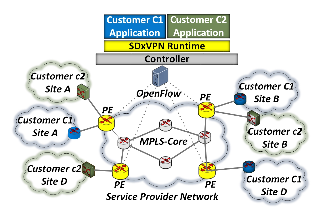
\includegraphics[scale=1.00]{sdxvpn_architecture}
	\centering
	\label{fig:sdxvpn_architecture}
\end{figure}
\begin{figure}[t]
	\caption{Modo de operación de cada servicio de acuerdo a su capa. Imagen extraída de \cite{sdxvpn}}
	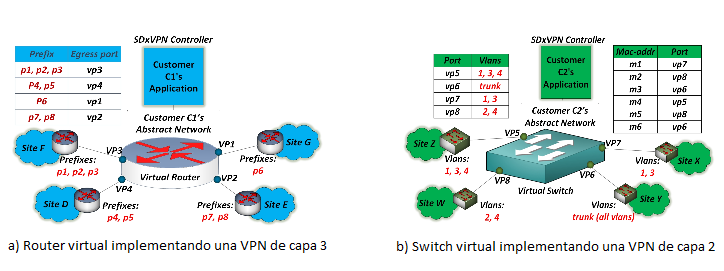
\includegraphics[scale=0.65]{sdxvpn_design}
	\centering
	\label{fig:sdxvpn_design}
\end{figure}
El diseño de la solución propuesta se puede ver en la figura \ref{fig:sdxvpn_architecture}. En la misma se observa la red de un hipotético proveedor de servicios conectada a dos clientes, cada uno con tres redes. La red del proveedor está dividida en dos partes: la región \textit{core} y los routers PE (Provider Edge). Este trabajo argumenta la necesidad enfoques híbridos SDN/Legacy, y es aquí donde lo aplica: si bien los routers PE son OpenFlow, el core de la red no utiliza SDN, y depende de LDP y Quagga para la distribución de etiquetas MPLS. Esto implica que los routers PE, además de utilizar OpenFlow, deben implementar Quagga y LDP. \\ \\
Otro dato importante que muestra la figura \ref{fig:sdxvpn_architecture} es la utilización de una aplicación por cada cliente. Esto permite proveer a los clientes un control personalizado sobre su servicio de VPN. Esas aplicaciones corren sobre una visión abstracta de la red, que depende de la capa del servicio. Si la VPN es de capa 3, el controlador SDxVPN ofrece un router virtual, y si es de capa 2 ofrece un switch virtual. Cada puerto en uno de estos dispositivos virtuales representa un puerto real de un dispositivo PE con un dispositivo CE (Customer Edge). Este enfoque le ofrece al cliente una visión abstracta de la red del proveedor, y se puede ver en la figura \ref{fig:sdxvpn_design}. En el caso de una VPN de capa 3, el cliente debe elegir un mecanismo de ruteo. Para el caso que muestra la figura, puede alcanzar con ruteo estático, pero para casos más complejos, el router virtual puede utilizar Quagga como motor. Todo esto implica que se construirá una tabla de ruteo virtual, la cual será traducida a flujos OpenFlow en los dispositivos PE. \\
Para la VPN de capa 2, el cliente debe asociar cada puerto del switch virtual con un conjunto de identificadores de VLAN. A ese mapeo se suma un mecanismo para aprender direcciones MAC (ya que debe comportarse como un switch de capa 2), y todo esto (igual que en la VPN de capa 3) se traduce en flujos OpenFlow que serán instalados en los dispositivos PE.

%http://yuba.stanford.edu/~nickm/papers/ofc11-saurav-mpls.pdf y http://klamath.stanford.edu/~nickm/papers/mpls-sigcomm11.pdf
\subsection{Otras aplicaciones}
En la sección anterior se presentaron algunas implementaciones de VPNs en SDN, que es la aplicación de más interés en este trabajo. A continuación se listan otras aplicaciones que se le puede dar a OpenFlow y SDN.
\begin{itemize}
	\item \textbf{Ingeniería de tráfico} es una disciplina que tiene como objetivo principal optimizar el rendimiento de una red. Una parte crucial de esta disciplina es poder monitorear en tiempo real el estado de cada elemento de la red. Esto es algo que OpenFlow resuelve, ya que puede registrar estadísticas por cada flujo, en tiempo real. Por ejemplo, en \cite{opennetmon} se presenta OpenNetMon, un módulo open source para el controlador POX que aprovecha las capacidades de monitoreo de OpenFlow y hace disponibles todas esas estadísticas para las aplicaciones que corren sobre el controlador. Una aplicación luego puede utilizar ese módulo y todas las estadísticas que provee para hacer ingeniería de tráfico, y tratar de optimizar los recursos de la red. \\
	El manejo de los flujos para lograr load balancing y la tolerancia a fallas son otros enfoques importantes, partes de la ingeniería de tráfico en SDN. En caso de que el lector desee profundizar en este tema, se recomienda la lectura de \cite{roadmap-sdn-te}, que hace un estudio completo de los enfoques actuales para la ingeniería de tráfico en redes OpenFlow.
	\item \textbf{Quality of Service}. Un problema muy común hoy en día es el de proveer distintos niveles de calidad de servicio, y SDN puede ser utilizado con ese propósito. El objetivo es aplicar distintos niveles de servicio a un determinado tráfico de acuerdo al cliente o al tipo de aplicación al que pertenece. Para lograr eso se pueden aplicar mecanismos como la reserva de recursos y el enrutamiento dinámico para cada flujo. \\
	Algunos ejemplos de trabajos hechos en este campo son: 1) FlowQoS \cite{flowqos}, una herramienta que permite a redes hogareñas reservar ancho de banda para cada tipo de tráfico mediante OpenFlow, 2) un framework basado en EuQoS \cite{euqos} para redes a gran escala, que utiliza OpenFlow para asignar prioridades a demanda a flujos de clientes. \\
	Si el lector desea profundizar en el tema de QoS sobre SDN, se recomienda la lectura de \cite{survey-sdn-qos}.
	\item \textbf{Detección y mitigación de ataques DoS}. Un controlador OpenFlow podría aprovechar las métricas y estadísticas ofrecidas por los switches OpenFlow para detectar, en tiempo real, ataques de denegación de servicio. El controlador también podría reaccionar ante el ataque, aplicando las entradas de flujos que correspondan para bloquear el tráfico utilizado, y así mitigar el efecto del ataque. Por ejemplo, Dossy \cite{openflow-dos-dossy} es una aplicación que corre sobre el controlador Beacon y permite detectar y mitigar ataques DoS. Analiza los mensajes packet\_in que recibe y las estadísticas de los flujos para detectar los ataques, y una vez los detecta, instala flujos para bloquear el tráfico atacante.
\end{itemize}

\section{Simuladores y emuladores}
El avance de las redes definidas por software ha motivado el desarrollo de nuevas herramientas que permitan la virtualización de este paradigma, para ayudar a los investigadores y administradores en el desarrollo y testing de sus arquitecturas. Como se explica en el capítulo 1, uno de los objetivos del proyecto es mover la arquitectura RAUFlow a una plataforma virtual. Por lo tanto, es importante hacer un estudio del estado del arte en lo que respecta a simuladores y emuladores de redes, con énfasis en los que contemplan el paradigma SDN.

La principal observación que se debe hacer es que ninguna de las herramientas estudiadas permite o contempla una naturaleza híbrida SDN/Legacy como la que plantea RAUFlow, donde los switches OpenFlow puedan comportarse como routers tradicionales. La tabla \ref{table:emuladores-y-simuladores} muestra las herramientas estudiadas. La segunda columna indica si la herramienta está orientada al concepto SDN. En las últimas dos columnas se pueden ver dos propiedades que aplican sólo a las herramientas orientadas a SDN. La penúltima indica la versión de OpenFlow que soporta, y la última indica si dicha herramienta puede ser utilizada con un controlador Ryu externo, en particular, el controlador RAUFlow.

La cuarta columna especifica si se trata de un emulador o simulador (en algunos casos se da que es un híbrido) y la quinta columna detalla cómo es el modo de virtualización que aplica la herramienta. Esta columna es de especial interés para analizar la escalabilidad de la herramienta. Si se trata de un motor de simulación o una emulación con virtualización ligera, es esperable que la herramienta pueda realizar experimentos con muchos nodos. Por otro lado, si utiliza máquinas virtuales completas para representar a los nodos, probablemente se trate de una herramienta diseñada para hacer experimentos chicos, con pocos nodos.

Las siguientes secciones estudian con más detalle las herramientas que se consideran más apropiadas para virtualizar la arquitectura RAUFlow/RAUSwitch. En la última sección se hace una mención aparte para un tipo de herramientas especial, que no sirve para hacer pruebas funcionales de una red como conjunto, sino que para hacer pruebas de estrés sobre cada elemento de la red por separado.

\begin{table}
\caption{Lista de emuladores y simuladores más relevantes para este trabajo.}
\centering
\resizebox{\textwidth}{!}{%
	\begin{tabular}{ | l | l | l | p{2.2cm} | p{4.0cm} | p{3.0cm} | p{2.8cm} |}
		\hline \hline
		\textbf{Herramienta} & \textbf{SDN} & \textbf{Open Source} & \textbf{Simulador o emulador} & \textbf{Modo de virtualización} & \textbf{OpenFlow} & \textbf{Permite Ryu/RAUFlow} \\ \hline
		Cloonix \cite{cloonix} & No & Si & Emulador & Máquinas virtuales completas & - & - \\ \hline
		CORE \cite{core} & No & Si & Emulador & Virtualización ligera (containers) & - & - \\ \hline
		DOT \cite{dot} & Si & Si & Emulador & Máquinas virtuales (hosts) y Open vSwitch (switches) & 1.3 (con Open vSwitch) & Si \\ \hline
		EstiNet \cite{estinet} & Si & No & Ambos & Simulación con mecanismos para ejecutar aplicaciones reales & 1.1.0 & Si \\ \hline
		FlowSim \cite{flowsim} & Si & Si & Simulador & Simulación & 1.3 & No \\ \hline
		fs-sdn \cite{fs-sdn} & Si & Si & Simulador & Simulación & No especifica versión & No \\ \hline
		GNS3 \cite{gns3} & No & Si & Ambos & Simulación con soporte para máquinas virtuales completas y ligeras & - & - \\ \hline
		IMUNES \cite{imunes} & No & Si & Emulador & Virtualización ligera (containers) & - & - \\ \hline
		Mininet \cite{mininet-paper} & Si & Si & Emulador & Virtualización ligera (containers) & 1.3 (con Open vSwitch) & Si \\ \hline
		MLN \cite{mln} & No & Si & Emulador & Máquinas virtuales completas & - & - \\ \hline
		Netkit \cite{netkit} & No & Si & Emulador & Máquinas virtuales completas & - & - \\ \hline
		NS-3 (extensión OpenFlow) \cite{ns-3-openflow} & Si & Si & Simulador & Simulación con mecanismos para ejecutar aplicaciones reales & 0.8.9 (con soporte para MPLS) & Posiblemente, pero sin confirmar \\ \hline
		Omnet++ (extensión OpenFlow) \cite{omnet-openflow} & Si & Si & Simulador & Simulación & 1.2 & No \\ \hline
		SDN Troubleshooting System \cite{sdn-troubleshooting-system} & Si & Si & Simulador & Simulación & 1.0 & Si \\ \hline
		Shadow \cite{shadow} & No & Si & Ambos & Simulación con mecanismos para ejecutar aplicaciones reales & - & - \\ \hline
		VNX \cite{vnx} & No & Si & Emulador & Máquinas virtuales completas / Virtualización ligera & - & - \\ \hline
	\end{tabular}}
	\label{table:emuladores-y-simuladores}
\end{table}

\subsection{DOT}
DOT (Distributed OpenFlow Testbed) \cite{dot} es un emulador open source distribuido de redes OpenFlow. Está diseñado para experimentos de gran escala, es decir, con muchos nodos. La idea principal es utilizar múltiples máquinas físicas para distribuir la carga de cómputo.

\begin{figure}[t]
	\caption{Arquitectura de gestión de DOT. Imagen extraída de \cite{dot}}
	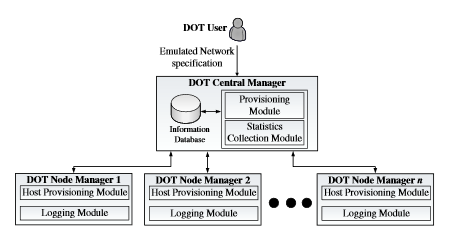
\includegraphics[scale=0.85]{dot_mgmt_arch}
	\centering
	\label{fig:dot_mgmt_arch}
\end{figure}

\begin{figure}[t]
	\caption{Arquitectura de cada nodo DOT físico. Imagen extraída de \cite{dot}}
	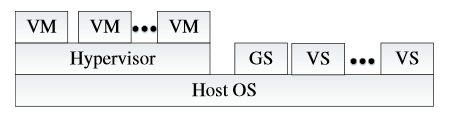
\includegraphics[scale=0.85]{dot_node_arch}
	\centering
	\label{fig:dot_node_arch}
\end{figure}

En la figura \ref{fig:dot_mgmt_arch} se puede ver la arquitectura de gestión de DOT. Se pueden distinguir dos tipos de componentes:
\begin{itemize}
	\item Central Manager. Este manejador (que puede estar en su propia máquina física) es responsable de gestionar los recursos para la red emulada indicada por el usuario. Está compuesto por dos módulos. El \textit{Provisioning Module} se encarga de ejecutar un algoritmo que decide cómo utilizar los recursos físicos (las máquinas físicas disponibles) de la manera más óptima para lograr emular la red deseada. Luego le comunica los resultados del algoritmo a cada nodo físico, para que cada uno sepa los recursos debe crear. El \textit{Statistics Collection Module} recolecta la información estadística que recibe de los nodos.
	\item Node Manager. Cada máquina física tiene uno, y está compuesto por dos módulos. El \textit{Host Provisioning Module} es responsable de instanciar y configurar los recursos que indica el manejador central. Esos recursos serán los hosts, switches y links virtuales. El \textit{Logging Module} recolecta estadísticas locales a cada nodo, como utilización de recursos, throughput, delay y mensajes OpenFlow.
\end{itemize}

La arquitectura interna de cada nodo físico en DOT se puede ver en la figura \ref{fig:dot_node_arch}. Los hosts virtuales (VM) son provistos por un hypervisor (KVM). En la figura también se observan múltiples switches virtuales (VS) que son implementados por Open vSwitch. Cada nodo físico también tiene un Gateway Switch (GS), que se encarga de reenviar paquetes entre switches virtuales alojados en distintas máquinas físicas. El Gateway Switch es transparente para el usuario.

\subsection{Estinet}
EstiNet \cite{estinet} es un emulador y simulador para redes OpenFlow, desarrollado por EstiNet Technologies Inc \footnote{http://www.estinet.com/ns/}.

\begin{figure}[H]
	\caption{Arquitectura de simulación de EstiNet. Imagen extraída de \cite{estinet}}
	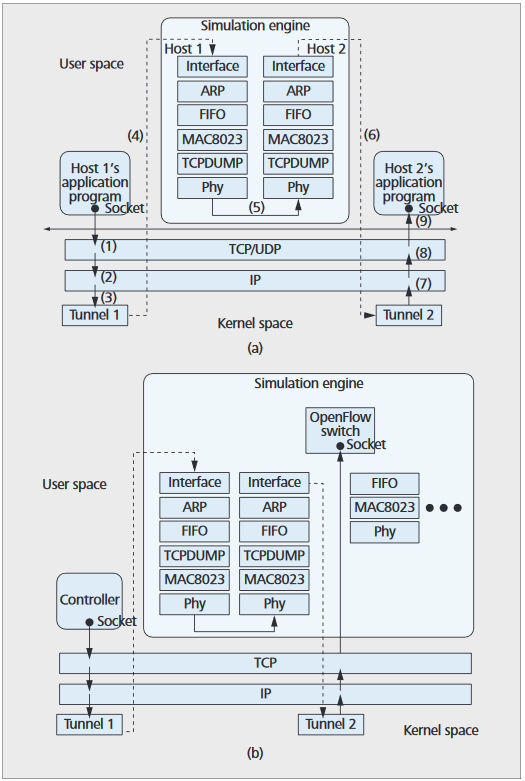
\includegraphics[scale=0.85]{estinet_simulation_archi}
	\centering
	\label{fig:estinet_simulation_archi}
\end{figure}

Gracias a una técnica llamada \textit{kernel re-entering}, EstiNet intenta combinar lo mejor de la simulación y emulación, para aprovechar sus ventajas y no sufrir las desventajas de cada una. El motor de simulación es capaz de simular hosts y switches OpenFlow, y utiliza interfaces de red de túnel para interceptar paquetes enviados entre aplicaciones reales. En la figura \ref{fig:estinet_simulation_archi}.a se puede ver como dos aplicaciones reales de Linux pueden ejecutar (desde cierto punto de vista) en dos hosts simulados, y conectarse entre sí. Cada host simulado es dotado con una interfaz y un stack de protocolos de capa 1 y 2. Las aplicaciones envían los paquetes a los hosts simulados mediante los túneles de Linux, luego los paquetes son enviados de un host a otro en el simulador y finalmente son entregados a la aplicación destinataria mediante su túnel correspondiente.

La figura \ref{fig:estinet_simulation_archi}.b muestra como se puede usar la misma técnica para permitir que controladores OpenFlow reales puedan comunicarse con los switches simulados. Un controlador es una aplicación que corre sobre Linux, por lo tanto se puede correr en un host simulado como muestra el ejemplo anterior. Un switch OpenFlow simulado puede utilizar una interfaz de túnel (en el ejemplo sería \textit{Tunnel 2}) para iniciar una conexión TCP OpenFlow con el controlador.

Este modo dual de EstiNet permite que se pueda integrar con aplicaciones reales, particularmente controladores OpenFlow reales, (algo que otros simuladores no pueden) y al mismo tiempo posea las ventajas de un simulador, como por ejemplo un reloj de simulación que garantiza la correctitud y precisión de los resultados que genera. Este enfoque también tiene ventajas en la escalabilidad, ya que se pueden conducir experimentos grandes a pesar de la limitación en el poder de cómputo de la computadora; el reloj del simulador se adecua al poder de cómputo disponible para asegurar la correctitud del experimento.

Una desventaja importante que tiene EstiNet es que, de acuerdo a \cite{estinet}, la versión máxima de OpenFlow que soporta es la 1.1.0, mientras que la versión que utiliza RAUFlow es la 1.3.1.

\subsection{Mininet}
Mininet es un emulador de redes SDN muy utilizado en la actualidad, que permite emular hosts, switches y enlaces. Utiliza \textit{virtualización ligera} en Linux para levantar una red completa en un único kernel. La virtualización ligera, también llamada virtualización en el nivel de sistema operativo, consiste en un conjunto de funcionalidades de Linux que le permiten a un sistema ser separado en múltiples \textit{containers} (contenedores) más chicos. Cada container tiene sus propios recursos, pero todos ejecutan sobre el mismo kernel, lo cual los hace más rápidos y livianos. Esto se combina con la capacidad de crear links virtuales entre dichos containers. Mininet no provee ni emula un controlador; el mismo se debe ejecutar como una aplicación común y corriente.

Este modo de funcionamiento logra que Mininet pueda ser mucho más rápido y escalable que emuladores que utilizan máquinas virtuales completas. Analizando con un poco más de detalle, a continuación se listan los componentes de Mininet y sus características:
\begin{itemize}
	\item Hosts. Un host emulado por Mininet es un grupo de procesos de usuario que ejecutan dentro de un \textit{network namespace}. Un network namespace le provee a un grupo de procesos sus propias interfaces de red, puertos, tablas de ruteo y tablas ARP.
	\item Enlaces. Los enlaces son emulados con virtual Ethernet (\textit{veth}), que actúa como un cable que conecta dos interfaces virtuales. Los paquetes enviados por una interfaz son recibidos por la otra, y cada interfaz virtual es vista como un puerto Ethernet totalmente funcional, tanto para el sistema como para las aplicaciones. El ancho de banda de los enlaces virtuales es controlado por Linux Traffic Control (\textit{tc}).
	\item Switches. Mininet puede utilizar el bridge de Linux o Open vSwitch para emular a los switches. El segundo es el que se utiliza para emular switches OpenFlow. Para emular múltiples switches OpenFlow se define un bridge por cada switch, todos ejecutándose en una única instancia de Open vSwitch. A diferencia de los hosts, que están en su propio network namespace, los switches de Open vSwitch comparten el root namespace, es decir, el namespace del sistema operativo. Como el controlador se ejecuta como una aplicación normal (no se ejecuta en un container ni tiene su propio network namespace), se puede comunicar con los switches mediante la interfaz de loopback del root namespace.
\end{itemize}

Mininet tiene una API en Python (el lenguaje en el que está escrito el emulador) que permite crear todo tipo de topologias. También tiene una línea de comandos que permite realizar acciones una vez la red virtual está levantada. Esas acciones pueden ser ejecutar un determinado comando en un host o switch, hacer una prueba de ping entre todos los hosts, etc.

Debido a su buena documentación y la forma en que está desarrollado, Mininet puede ser fácilmente extensible para lograr experimentos que la versión estándar no contempla. Existen diversos trabajos donde se presentan extensiones a Mininet, para lograr objetivos específicos:
\begin{itemize}
	\item Mininet-HiFi \cite{mininet-hifi} intenta mejorar el realismo de la emulación en Mininet, agregando mecanismos de reserva de recusos y monitoreo para los mismos.
	\item MaxiNet \cite{maxinet} y Mininet CE \cite{mininet-ce} son extensiones para hacer emulaciones distribuidas, es decir, con múltiples máquinas físicas.
	\item Mininet DC \cite{mininet-dc} es un trabajo que extiende Mininet y el controlador POX para hacer experimentos orientados a data centers en la nube.
\end{itemize}
\subsection{NS-3}
NS-3 es un simulador de redes open source basado en eventos discretos. Es una herramienta desarrollada para ser extensible por módulos escritos por los usuarios. Es por esta característica que puede ser utilizada para usar OpenFlow, a pesar de no ser una herramienta enfocada hacia el paradigma SDN.

Existe una implementación de OpenFlow \cite{ns-3-openflow} (llamada OFSID - \textit{OpenFlow software implementation distribution}) que se puede integrar con ns-3 en modalidad de librería externa. Esta extensión implementa una versión antigua de OpenFlow, la 0.8.9, pero agrega soporte para MPLS.

Un problema de esta extensión es que la entidad controlador es modelada internamente en el simulador. Esto implica que no es posible que el simulador funcione con un controlador externo. Esto podría resolverse con una funcionalidad llamada \textit{Direct Code Execution} (DCE), que permite la ejecución de aplicaciones externas dentro de ns-3. Sin embargo, DCE sólo soporta, de forma oficial, aplicaciones C/C++, y el soporte para Python por el momento es experimental.

Otro detalle importante es que no es posible modelar la conexión SSL entre un switch OpenFlow y el controlador (ya que es interno). Esto baja la calidad de la simulación ya que podría ser un punto interesante de estudio.

En resumen, NS-3 es un simulador muy usado en la actualidad pero su soporte para redes OpenFlow podría etiquetarse como experimental por el momento. Es necesario hacer un estudio muy detallado para determinar si se puede utilizar con la arquitectura RAUFlow, pero no se descarta que así sea.

\subsection{IMUNES y otros emuladores de propósito general}
IMUNES \cite{imunes} es un emulador open source para Linux y FreeBSD. Funciona con nodos virtuales ligeros (o containers) conectados entre sí por enlaces emulados.

Para implementar redes virtuales en Linux usa dos tecnologías: Docker y Open vSwitch. Docker es una herramienta open source que utiliza virtualización a nivel de sistema operativo (o virtualización ligera) para crear \textit{containers}. Estos nodos virtuales o \textit{containers} son muy similares a los que implementa Mininet, y tienen como gran ventaja que son mucho más rápidos y utilizan menos recursos que las máquinas virtuales completas.

IMUNES es similar a otras herramientas que usan virtualización ligera como VNX \cite{vnx}, CORE \cite{core} y GNS3 \cite{gns3}. Son opciones bastante más escalables que otros emuladores como Cloonix \cite{cloonix}, MLN \cite{mln} y Netkit \cite{netkit}, que utilizan máquinas virtuales completas.

\subsection{Herramientas para pruebas de estrés y benchmarking}
Existen múltiples herramientas de testing aplicables en el paradigma SDN. De ellas se puede destacar un grupo, que no tienen como objetivo verificar aspectos funcionales, sino que apuntan a algo mucho más específico: las pruebas de estrés y el benchmarking. Ayudan a los administradores de red e investigadores a conocer los niveles de rendimiento de los cuales sus dispositivos y controladores son capaces. Asimismo, pueden ser elementos de investigación útiles en el contexto de la nueva Red Académica, ya que podrían utilizarse, por ejemplo, para validar ciertos aspectos de rendimiento de los RAUSwitch.

En esta sección se estudiarán algunos ejemplos de estas herramientas, agrupándolas en dos grupos, de acuerdo a la entidad que intentan probar: switches y controladores. Para mantener la relevancia con el contexto de este trabajo, se limitará a herramientas enfocadas a OpenFlow. \\ \\
\textbf{Testing de switches} \\
El testing y benchmarking de switches OpenFlow tiene como objetivo analizar cuál es el nivel máximo de rendimiento que puede alcanzar un switch. Esto por lo general se logra simulando las condiciones de una red que está bajo mucha carga, y sometiendo al switch a dichas condiciones, monitoreando su comportamiento. A continuación se listan algunas herramientas que hacen esto:
\begin{itemize}
	\item \textbf{OFLOPS} \cite{oflops} (OpenFlow Operations Per Second) es un framework open source para el testing y benchmarking de switches OpenFlow, tanto físicos como virtuales. Está desarrollado en el lenguaje C, y utiliza librerías de manipulación de paquetes para emular un controlador OpenFlow y tráfico de uso. Fue diseñado con un enfoque multi-thread para aprovechar las arquitecturas multi-core y así aumentar la potencia de la plataforma. Consiste de cinco threads paralelos, cada uno cumpliendo una función específica: 1) generación de paquetes, 2) captura de paquetes, 3) administración del canal de control (mensajes OpenFlow), 4) administración de un canal SNMP para hacer consultas asíncronas, y 5) un manejador de tiempo. Todo esto lo ofrece mediante una API, permitiendo a los usuarios crear sus propios módulos para escribir pruebas que se adapten a su realidad.
	\item \textbf{Spirent OpenFlow Controller Emulation} \cite{spirent-controller-emulation} es una herramienta desarrollada por la empresa Spirent\footnote{http://spirent.com/} que, igual que OFLOPS, tiene como propósito el testing y benchmarking de switches OpenFlow. Puede emular un controlador OpenFlow, definir millones de flujos y aplicar patrones de tráfico a esos flujos, y de ese modo medir el rendimiento, disponibilidad, seguridad y escalabilidad del switch. Entre sus funcionalidades, se destaca que puede probar todos los aspectos de OpenFlow 1.3, y que puede trabajar con switches híbridos. Estos dos puntos lo hacen una valiosa herramienta para el testing del RAUSwitch.
\end{itemize}
\textbf{Testing de controladores} \\
Similar al caso de los switches, las pruebas de estrés sobre controladores OpenFlow consisten en someterlos a condiciones de mucha carga y estudiar determinadas métricas de su comportamiento. En general los principales aspectos que se buscan estudiar son 1) la cantidad de sesiones paralelas con switches OpenFlow que puede mantener el controlador y 2) el ritmo de mensajes packet\_in que puede manejar. No sólo es útil conocer esos umbrales, sino que también es muy valioso saber cual es el comportamiento esperado si se exceden dichos umbrales. Al ser RAUFlow un controlador de estilo proactivo, el aspecto número dos no es relevante aquí, ya que la red no genera paquetes de tipo packet\_in. A continuación se listan algunas de las herramientas disponibles:
\begin{itemize}
	\item \textbf{Cbench} \cite{cbench} es una herramienta para benchmarking de controladores, y es parte del proyecto OFLOPS. Su funcionamiento es muy simple: el usuario indica una cantidad \textit{n} de switches, la herramienta crea \textit{n} sesiones OpenFlow paralelas con el controlador, y luego comienza a enviar mensajes de tipo packet\_in y mide el tiempo que demora el controlador en responder a esos mensajes.
	\item \textbf{Spirent OpenFlow Switch Emulation} \cite{spirent-switch-emulation} es la propuesta de Spirent para el stress-testing de controladores OpenFlow. Igual que Cbench, en esencia consiste en emular múltiples switches y generar mensajes de tipo packet\_in. Sin embargo, es una solución un poco más sofisticada que Cbench, ya que permite trabajar con múltiples topologias y protocolos como ARP y LLDP.
\end{itemize}


